\documentclass{article}

\usepackage[utf8]{inputenc}
\usepackage[brazilian]{babel}
\usepackage{graphicx}
\usepackage{float}
\usepackage[pdftex]{hyperref}
\usepackage{epstopdf}
\usepackage{etoolbox}
\usepackage{amsmath}
\usepackage{amsfonts}
\usepackage{amssymb}
\usepackage{caption}
\usepackage{subcaption}
\usepackage{setspace}
\usepackage{tikz}

\patchcmd{\thebibliography}{\section*}{\section}{}{}
\newcommand{\R}{\ensuremath{\mathbb{R}}}
\newcommand{\Prob}{\ensuremath{\mathbb{P}}}
\newcommand{\K}{\ensuremath{\mathbb{K}}}
\newcommand{\U}{\ensuremath{\mathbb{U}}}
\newcommand{\N}{\ensuremath{\mathbb{N}}}
\newcommand{\Lg}{\ensuremath{\mathbb{L}}}
\newcommand{\T}{\ensuremath{\rm Tr}}
\newcommand{\sg}{{\sigma(x_k)}}

\newcommand{\G}{\ensuremath{\mathcal{G}}}
\newcommand{\F}{\ensuremath{\mathcal{F}}}
\newcommand{\C}{\ensuremath{\mathcal{C}}}
\newcommand{\E}{\ensuremath{\mathcal{E}}}
\newcommand{\Hn}{\ensuremath{\mathcal{H}}}
%\newcommand{\Hoo}{\ensuremath{\mathcal{H}_\infty}}
\newcommand{\Hop}{\ensuremath{\mathcal{H}_{op}}}
% --------------------------------------------------
\newtheorem{theo}{Teorema}
\newtheorem{exa}{Exemplo}
\newtheorem{lemm}{Lema}
\newtheorem{coro}{Corolário}
\newtheorem{defn}{Definição}[section]

%opening


\begin{document}

\begin{titlepage}
\begin{center}

\newcommand{\HRule}{\rule{\linewidth}{0.5mm}}
% Upper part of the page. The '~' is needed because \\
% only works if a paragraph has started.

\includegraphics[width=0.15\textwidth]{logounicamp.pdf}~\\[1cm]

\textsc{\LARGE Universidade Estadual de Campinas}\\[1.5cm]

\textsc{\Large Faculdade de Engenharia Mecânica}\\[0.5cm]

% Title
\HRule \\[0.4cm]
{ \huge \bfseries ES828 - Laboratório de Controle de Sistemas\\ \vspace{1cm} Relatório - Experimento 2 \\
\Large{Método de identificação de plantas eletrônicas} \\[0.4cm] }

\HRule \\[1.5cm]

% Author and supervisor
\begin{minipage}{0.6\textwidth}
\begin{flushleft} \large
\emph{Nome:}\\
Daniel Dello Russo Oliveira\\ Marcelli Tiemi Kian
\end{flushleft}
\end{minipage}
\begin{minipage}{0.2\textwidth}
\begin{flushright} \large
\emph{RA}\\ 101918\\
117892
\end{flushright}
\end{minipage}

\vfill

% Bottom of the page
{\large \today}

\end{center}
\end{titlepage}


\onehalfspacing
\section{Objetivos} 
O objetivo desse experimento é a familiarização com o estudo do projeto de controladores PID analógicos utilizando resistores, capacitores e amplificadores operacionais. 
	
\section{Projeto do Controlador Analógico}
Consideramos a planta cuja função de transferência representada pela equação \ref{eq:gs} que foi obtida usando as medidas realizadas durante o experimento 2, consideramos também o controlador PID do experimento 3 obtido pelo método de Ziegler-Nichols mostrado na equação \ref{eq:pidz} que se mostrou melhor que o projetado com auxílio da ferramenta SISOTool do Matlab mostrado na equação \ref{eq:pids}.\\

\begin{equation}
\label{eq:gs}
G(s) = \frac{\kappa_1*\kappa_2*\kappa_3*\kappa_4}{(s*\tau_2 + 1)(s*\tau_3 + 1)s}
\end{equation}

\begin{table}[H]
\centering
\caption{Parâmetros numéricos da função de transferência}
\label{tab:valores}
\begin{tabular}{|c|c|}
	\hline Componente & Valor \\ 
	\hline $\kappa_1$ & $-0.1005$\\ 
	\hline $\kappa_2$ & $-2.1508$\\ 
	\hline $\kappa_3$ & $-4.6448$\\ 
	\hline $\kappa_4$ & $-5.6307$\\ 
	\hline $\tau_2$ & $0.0210$\\ 
	\hline $\tau_3$ & $0.0244$ \\ 	
	\hline 
\end{tabular} 
\end{table}

\begin{equation}
\label{eq:pidz}
K_z(s) = 9.05+\frac{142}{s}+0.144 s
\end{equation}

\begin{equation}
\label{eq:pids}
K_s(s) = 5.3+\frac{2.37}{s}+0.207 s
\end{equation}

\subsection{Circuito do controlador PID analógico}
Utilizando o modelo proposto no roteiro \cite{bb:roteiro} mostrado na figura \ref{fig:circuito} com a aproximação mostrada na equação \ref{eq:kpkikd}, podemos determinar os valores de $R_1$, $R_2$ e $R_3$ dado que foi fixado $C=1 \mu F$ para obter os desejados valores de $\kappa_p$, $\kappa_i$ e $\kappa_d$.

\begin{figure}[H]
	\centering
	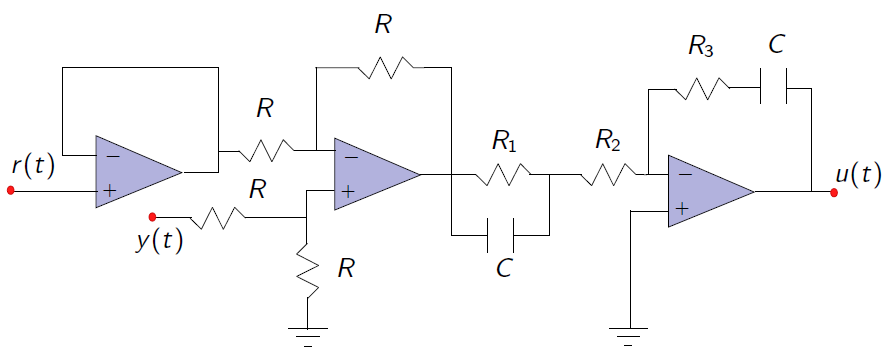
\includegraphics[width=\linewidth]{circuito}
	\caption{Circuito analógico para controlador PID}
	\label{fig:circuito}
\end{figure}

\begin{equation}
\label{eq:kpkikd}
\frac{\kappa_d s^2+\kappa_p s+\kappa_i}{s} \approx \frac{\frac{R_1 R_3 C}{R_1 + R_2} s^2 + \frac{R_1 + R_3}{R_1 + R_2} s+\frac{1}{R_1 + R_2}}{\frac{R_1 R_2 C}{R_1 + R_2}s^2 +s} 
\end{equation}

\subsection{Determinação dos resistores}
Inicialmente, a partir dos parâmetros do controlador obtido por Ziegler-Nichols da equação \ref{eq:pidz} tentamos resolver o sistema de equações que levasse aos valores indicados de resistores, mas não encontramos nenhuma solução plausível, pois não devem ser consideradas resistências negativas ou que sejam maiores do que poucos Mega-Ohms. \\

Partimos então para uma abordagem diferente, entendendo como a alteração dos valores de cada um dos três resistores afetavam os parâmetros do controlador. A partir disso, utilizamos um método iterativo para nos aproximar ao máximo dos parâmetros desejados, mas não conseguimos encontrar valores satisfatoriamente aproximados. A cada ajuste, um parâmetro diferente não saía da faixa desejável. Ainda assim, tentamos simular um novo controlador baseado no projetado por Ziegler-Nichols e não obtivemos uma boa resposta.\\

Retomamos então o controlador projetado pelo SISOTool no experimento anterior, mostrado na equação \ref{eq:pids}, que apresentou resultados em laboratório piores que o projetado por Ziegler-Nichols, porém acreditamos que grande parte dos problemas que encontramos nesse experimento se devem ao fato do controlador implementado ter sido digital. Conseguimos fazer uma boa aproximação dos seus parâmetros utilizando os valores de resistores disponíveis, também de maneira iterativa, chegando aos valores de $R_1=51k\Omega$,$R_2=1.5k\Omega$ e $R_3=200k\Omega$, que levam a valores aproximados de $\kappa_p=4.78$, $\kappa_i=19.05$ e $\kappa_d=0.194$. Como podemos ver, para manter $\kappa_p$ e $\kappa_d$ semelhantes ao projetado anteriormente, $\kappa_i$ acabou ficando maior.\\

Nas simulações a seguir observamos que, mesmo com valores predefinidos de resistores e sem utilizar o artifício de ligá-los em série ou paralelo para criar novos valores de resistência, é possível se aproximar dos valores calculados e obter resultados satisfatórios.
A primeira simulação (figura \ref{fig:yrsimpidstep}) mostra a saída e entrada, para o controlador analógico encontrado e a figura \ref{fig:rusimpidstep} mostra o seu esforço de controle. A entrada nessa simulação é uma onda quadrada de amplitude de $1V$ e frequência de $0.25Hz$. Podemos ver que o esforço de controle apresenta um pico que ultrapassa os $10V$ definidos no momento das transições, esse pico se deve principalmente à ação do termo derivativo do controlador, como nas transições a derivada da entrada é infinita.

\begin{figure}[H]
	\centering
	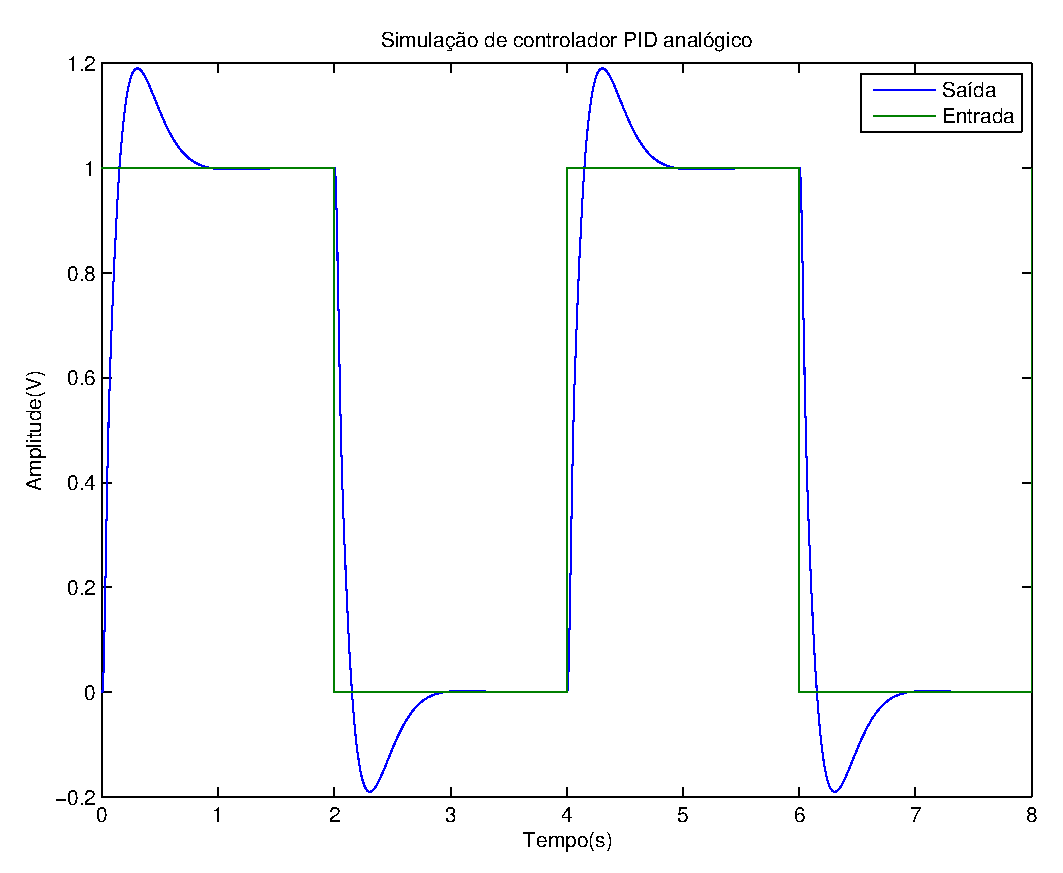
\includegraphics[width=0.8\linewidth]{yr1000step}
	\caption{Simulação do controlador PID analógico para onda quadrada}
	\label{fig:yrsimpidstep}
\end{figure}
\begin{figure}[H]
	\centering
	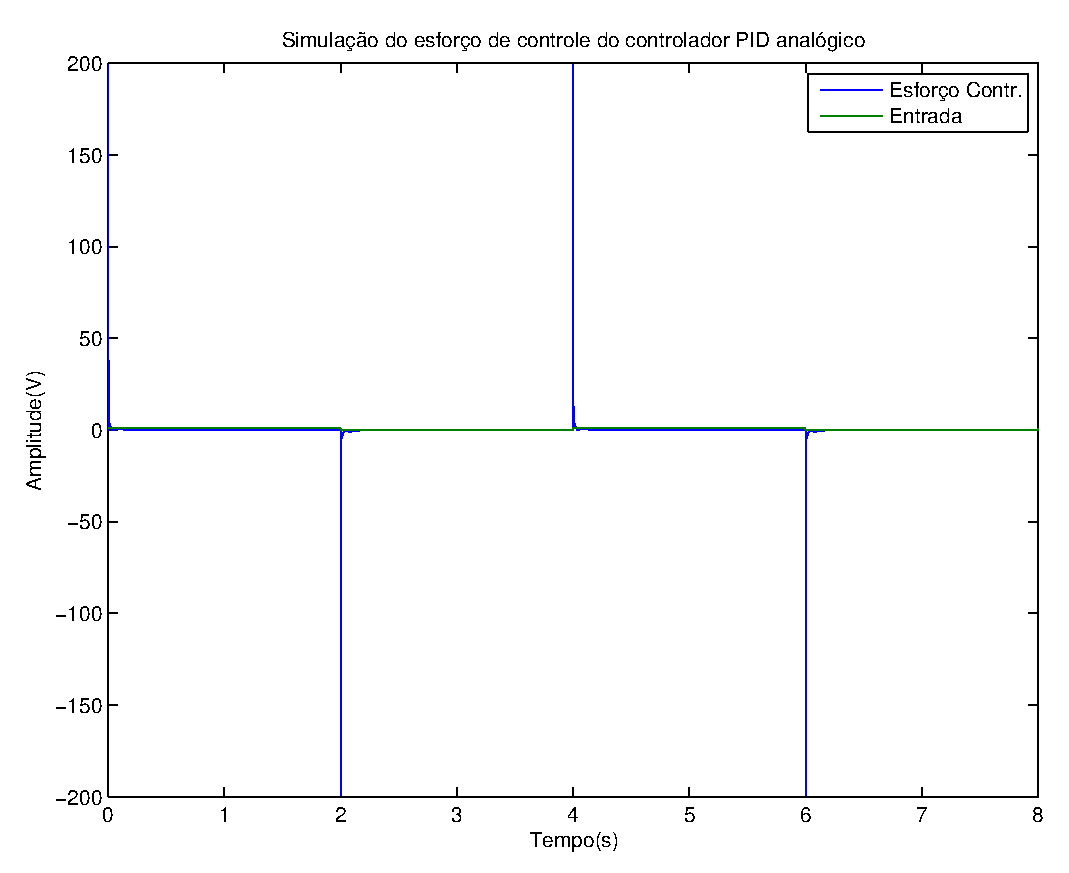
\includegraphics[width=0.8\linewidth]{ru1000step}
	\caption{Esforço de controle simulado do controlador PID analógico para onda quadrada}
	\label{fig:rusimpidstep}
\end{figure}

Para solucionar esse problema suavizamos as transições da entrada, se aproximando mais de um sistema real, utilizando uma função seno de amplitude $10V$ e período de $0.25Hz$, com saturação em $1V$, como podemos ver na figura \ref{fig:yrusimpid} o esforço de controle cai então para dentro da faixa desejada. 
\begin{figure}[H]
\centering
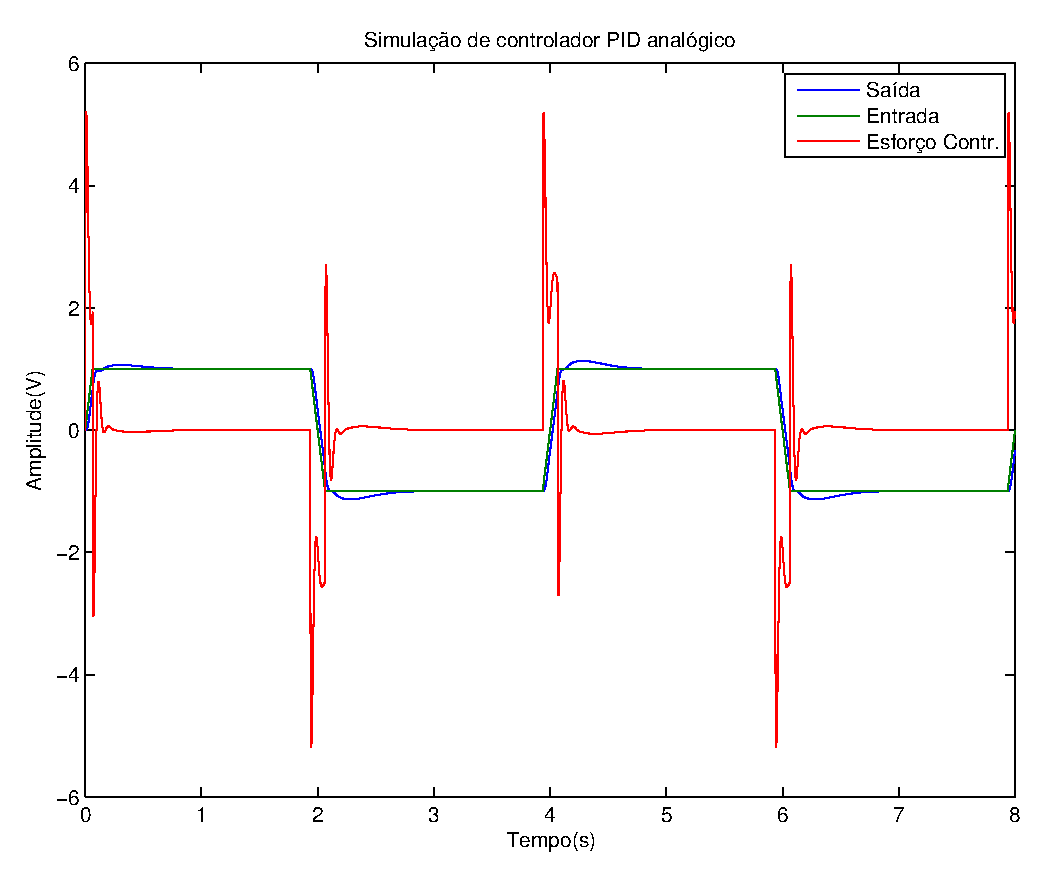
\includegraphics[width=0.8\linewidth]{yru1000sin}
\caption{Simulação do controlador PID analógico para onda quadrada suavizada}
\label{fig:yrusimpid}
\end{figure}

Por fim, para nos aproximar mais de um sistema real, diminuímos o coeficiente de filtro do derivador, afastando um dos polos do infinito. Simulamos também esse sistemas e vimos que a resposta continua aceitável, como pode ser visto na figura \ref{fig:yrusimpid100}.
\begin{figure}[H]
	\centering
	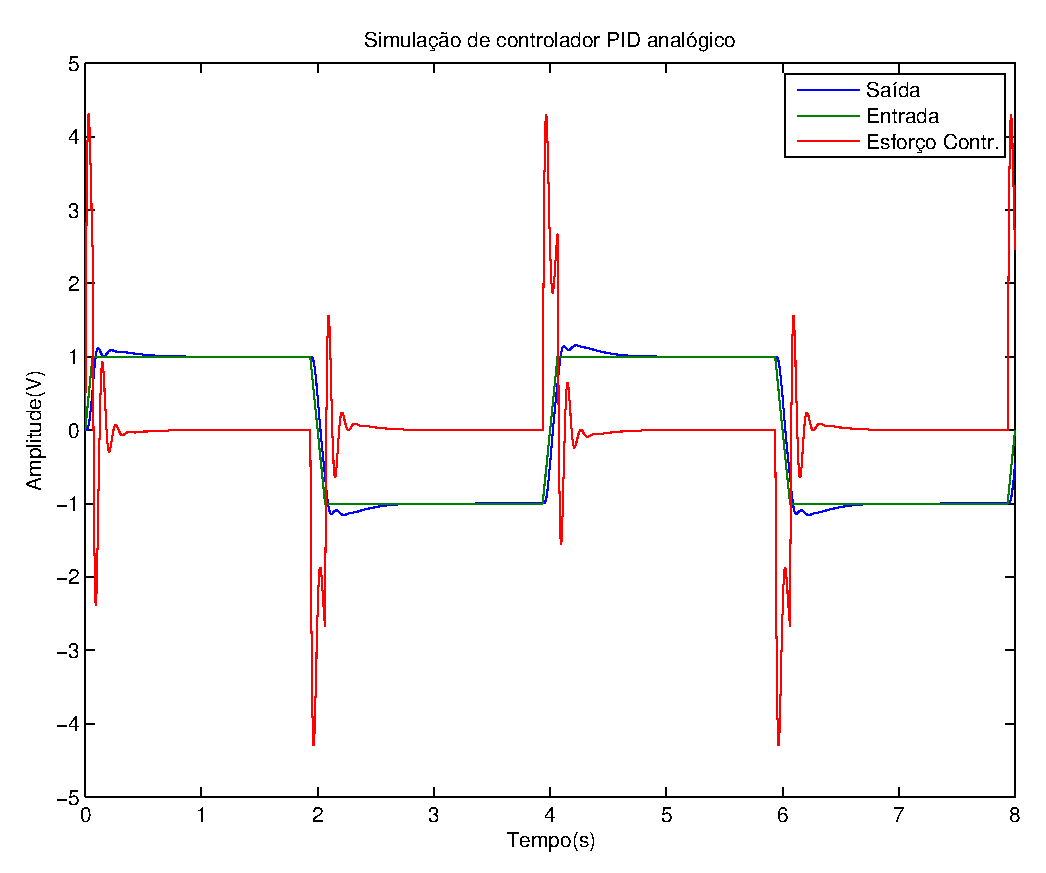
\includegraphics[width=0.8\linewidth]{yru100sin}
	\caption{Simulação do controlador PID analógico realista para onda quadrada suavizada}
	\label{fig:yrusimpid100}
\end{figure}

Comparando essa simulação com o resultado obtido no relatório do experimento 3 \cite{bb:lab3}, mostrado na figura \ref{fig:ypids2}, podemos ver que o resultado simulado é significativamente superior. Esperamos conseguir algo semelhante implementando o controlador de maneira analógica, uma vez que esse será menos suscetível aos ruídos introduzidos pela aquisição. 
\begin{figure}[H]
	\centering
	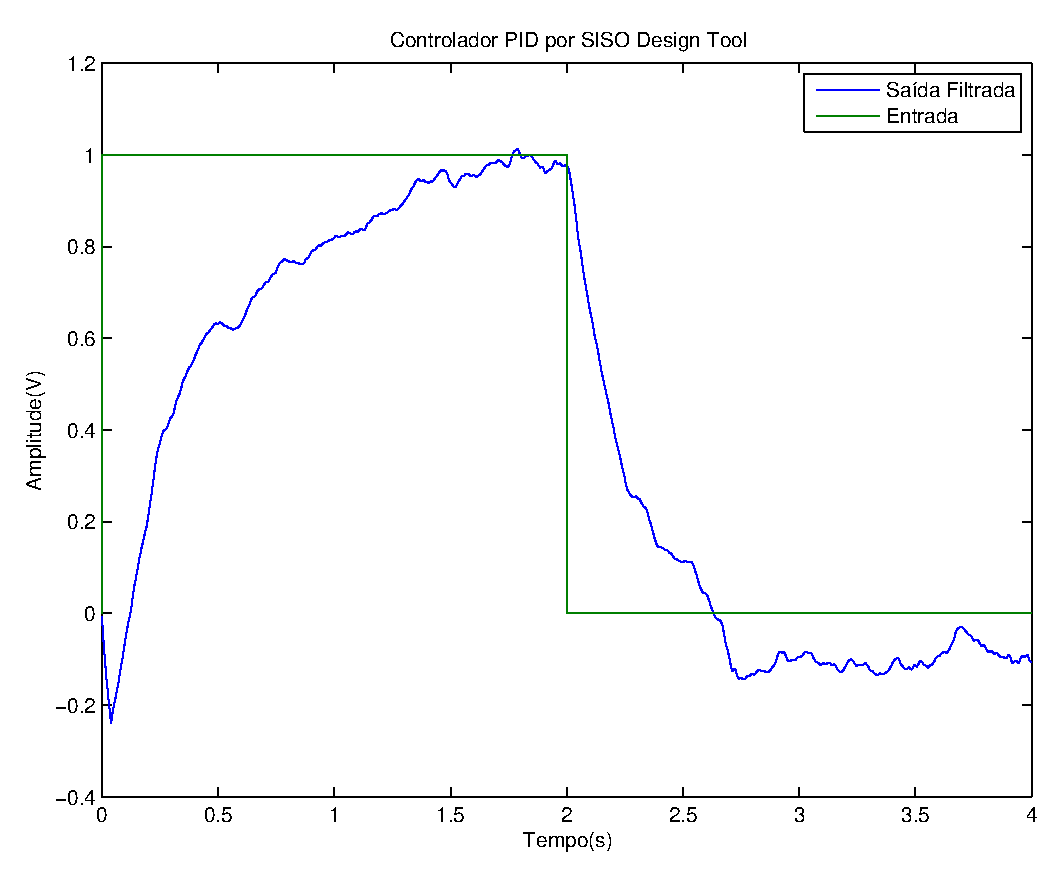
\includegraphics[width=0.8\linewidth]{ypids2}
	\caption{Resposta do controlador PID digital para onda quadrada}
	\label{fig:ypids2}
\end{figure}
Comparamos também o controlador analógico simulado com a simulação do controlador projetado originalmente, vista na figura \ref{fig:yusimpids}, e vimos que ao aumentar o valor de $\kappa_i$, introduzimos uma sobrelevação significativa na resposta e também deslocamos seu tempo de estabilização. Porém acreditamos que esse controlador continua aceitável e, conforme observamos na implementação digital do controlador original, essa simulação não representa bem a realidade do sistema.
\begin{figure}[H]
	\centering
	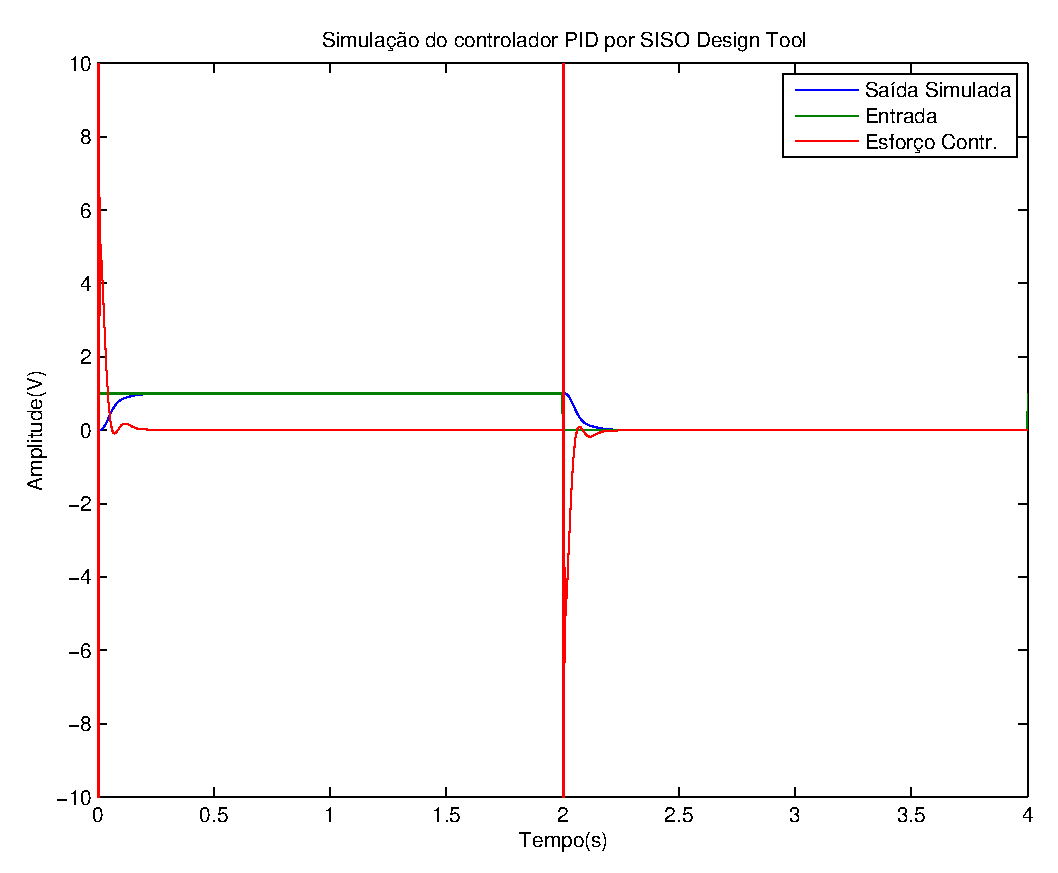
\includegraphics[width=0.8\linewidth]{yusimpids}
	\caption{Resposta simulada do controlador PID digital para onda quadrada}
	\label{fig:yusimpids}
\end{figure}
\begin{thebibliography}{widestlabel}
	\bibitem{bb:roteiro}{Roteiro do experimento disponibilizado para os alunos}
	\bibitem{bb:lab3}{KIAN, Marcelli; OLIVEIRA, Daniel. \textit{Relatório - Experimento 3:} Controle de plantas eletrônicas utilizando um controlador PID digital.}
\end{thebibliography}
\end{document}

